\documentclass[a4paper,11pt,dvipdfmx]{jsarticle}

\usepackage{url}

% 数式
\usepackage{amsmath,amsfonts}
\usepackage{bm}

% 画像
\usepackage[dvipdfmx]{graphicx}
\usepackage{framed}

% 図形
\usepackage{tikz}
\usepackage{pgfplots}
\usepackage[european]{circuitikz}
\usepackage{etoolbox}

\AtBeginEnvironment{tikzpicture}{\small}
\pgfplotsset{compat=1.18}
\usetikzlibrary{shapes.geometric}
\usetikzlibrary {shapes.misc}

% ソースコード
\usepackage{listings,jlisting,color}
\lstset{
language={Python},
backgroundcolor={\color[gray]{.85}},
basicstyle={\ttfamily},
identifierstyle={\small},
commentstyle={\small \color[rgb]{0,0.5,0}},
keywordstyle={\small\bfseries \color[rgb]{0.5,0,0.5}},
ndkeywordstyle={\small},
stringstyle={\small\ttfamily \color[rgb]{0,0,1}},
frame={tb},
breaklines=true,
columns=[l]{fullflexible},
numbers=left,
xrightmargin=0zw,
xleftmargin=3zw,
numberstyle={\scriptsize},
stepnumber=1,
numbersep=1zw,
lineskip=-0.5ex,
}
\renewcommand{\lstlistingname}{ソースコード}

\begin{document}
\begin{titlepage}
\noindent
\vspace{4cm}
\begin{center}
\begin{LARGE}
組込システムI \\
第5回  課題 \\
\vspace{8cm}
提出日  2025/05/22 \\
学籍番号  21T2166D \\
名前  渡辺 大樹 \\
\end{LARGE}
\end{center}
\end{titlepage}

\definecolor{shadecolor}{gray}{0.70}

\section{演習2 - ADコンバータによる分圧測定}
\begin{shaded}
    \noindent
    資料の回路を作成して、抵抗による分圧電圧をADコンバータで読み込み、理論値と比較せよ。
    \begin{itemize}
        \item 抵抗値は、2k, 6.8k, 33k, 47kの4種類の組み合わせを比較する。
        \item 分圧電圧は、Vout=Vin×R2/(R1+R2)で求める。
        \item ADコンバータの分解能は、10bitである。
    \end{itemize}
\end{shaded}

\subsection{回路}
以下に実装した回路の写真と回路図を示す。
\begin{figure}[h]
    \centering
    \includegraphics[width=100mm]{c:/Program_Code/LaTeX/BuiltIn/exam5/PXL_20250522_063605566.jpg}
    \caption{演習2 回路の写真 (MCP3002 と固定抵抗による分圧)}
    \label{fig:exam2-photo}
\end{figure}

\begin{figure}
    \centering
    \scriptsize % Reduce font size for this figure
    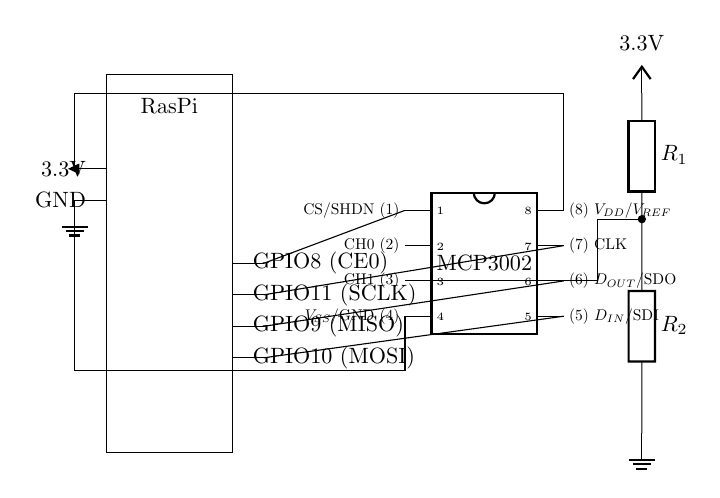
\begin{tikzpicture}[scale=0.8, transform shape]
        \ctikzset{label/align = smart}

        % Raspberry Pi (Simplified)
        \draw (0,0) rectangle (2,6);
        \node at (1,5.5) {RasPi};

        \node[anchor=east] at (-0.2, 4.5) {3.3V}; \draw (0,4.5) -- ++(-0.5,0) node[currarrow,rotate=180]{};
        \node[anchor=east] at (-0.2, 4.0) {GND}; \draw (0,4.0) -- ++(-0.5,0) node[ground]{};

        \node[anchor=west] at (2.2, 3.0) {GPIO8 (CE0)}; \draw (2,3.0) -- ++(0.5,0);
        \node[anchor=west] at (2.2, 2.5) {GPIO11 (SCLK)}; \draw (2,2.5) -- ++(0.5,0);
        \node[anchor=west] at (2.2, 2.0) {GPIO9 (MISO)}; \draw (2,2.0) -- ++(0.5,0);
        \node[anchor=west] at (2.2, 1.5) {GPIO10 (MOSI)}; \draw (2,1.5) -- ++(0.5,0);

        % MCP3002 (DIP-8 style)
        \node (mcp3002) [dipchip, num pins=8, external pins width=0.3] at (6,3) {MCP3002};
        \node[anchor=east, scale=0.7] at (mcp3002.pin 1) {CS/SHDN (1)};
        \node[anchor=east, scale=0.7] at (mcp3002.pin 2) {CH0 (2)};
        \node[anchor=east, scale=0.7] at (mcp3002.pin 3) {CH1 (3)};
        \node[anchor=east, scale=0.7] at (mcp3002.pin 4) {$V_{SS}$/GND (4)};
        \node[anchor=west, scale=0.7] at (mcp3002.pin 5) {(5) $D_{IN}$/SDI};
        \node[anchor=west, scale=0.7] at (mcp3002.pin 6) {(6) $D_{OUT}$/SDO};
        \node[anchor=west, scale=0.7] at (mcp3002.pin 7) {(7) CLK};
        \node[anchor=west, scale=0.7] at (mcp3002.pin 8) {(8) $V_{DD}$/$V_{REF}$};

        % Connections: Raspberry Pi to MCP3002
        % Route 3.3V to VDD/VREF (pin 8)
        \draw (-0.5, 4.5) -- ++(0,1.2) node[coordinate](vcc_bus){} -| (mcp3002.pin 8);
        % Route GND to VSS/GND (pin 4)
        \draw (-0.5, 4.0) -- ++(0,-2.7) node[coordinate](gnd_bus){} -| (mcp3002.pin 4);

        \draw (2.5, 3.0) -- (mcp3002.pin 1); % CE0 to CS
        \draw (2.5, 2.5) -- (mcp3002.pin 7); % SCLK to CLK
        \draw (2.5, 2.0) -- (mcp3002.pin 6); % MISO to DOUT
        \draw (2.5, 1.5) -- (mcp3002.pin 5); % MOSI to DIN

        % Voltage Divider for Exercise 2
        \coordinate (vcc_ex2) at (8.5, 5.7); % Adjusted position for clarity
        \coordinate (gnd_ex2) at (8.5, 0.3); % Adjusted position for clarity
        \draw (vcc_ex2) node[vcc]{3.3V} to[R, l=$R_1$] ++(0,-2) coordinate (r1r2_jct);
        \draw (r1r2_jct) to[R, l=$R_2$] (gnd_ex2) node[ground]{};
        \node[circ] at (r1r2_jct) {};
        \draw (r1r2_jct) -- ++(-0.7,0) |- (mcp3002.pin 3); % Junction to CH1, adjusted routing
        \node[anchor=south, scale=0.7] at (mcp3002.pin 3) {}; % ensure label space isn't overwritten
       
        % CH0 not connected or to GND (showing not connected as per slide style)
        % \draw (mcp3002.pin 2) -- ++(-0.3,0) node[xmittale, scale=0.5]{}; % NC symbol
    \end{tikzpicture}
    \caption{演習2 回路図 (MCP3002 と固定抵抗による分圧)}
    \label{fig:exercise2_updated}
\end{figure}

\subsection{プログラム}
ソースコード\ref{exam5-2}に分圧測定を行ったプログラムを示す。
このコードでは、ADコンバータを使用して分圧電圧を測定している。

測定部分で0.5秒おきにADコンバータの値を取得し、それの10回合計を取ってから平均値を計算している。

\subsection{実行結果}
以下に実行結果を示す。
\begin{table}[htbp]
    \centering
    \caption{固定抵抗による分圧電圧測定結果}
    \begin{tabular}{|c|c|c|c|c|c|}
        \hline
        \textbf{$R_1$ [Ω]} & \textbf{$R_2$ [Ω]} & \textbf{ADC値} & \textbf{測定電圧 [V]} & \textbf{理論電圧 [V]} & \textbf{誤差 [\%]} \\
        \hline
        2,000 & 47,000 & 982.2 & 3.17 & 3.13 & 1.28 \\
        \hline
        2,000 & 6,800 & 817.5 & 2.64 & 2.61 & 1.15 \\
        \hline
        2,000 & 33,000 & 983.0 & 3.17 & 3.06 & 3.59 \\
        \hline
        6,800 & 2,000 & 231.0 & 0.75 & 0.75 & 0.00 \\
        \hline
        6,800 & 33,000 & 849.7 & 2.74 & 2.72 & 0.74 \\
        \hline
        6,800 & 47,000 & 893.6 & 2.88 & 2.86 & 0.70 \\
        \hline
        33,000 & 6,800 & 173.4 & 0.56 & 0.56 & 0.00 \\
        \hline
        33,000 & 2,000 & 59.2 & 0.19 & 0.19 & 0.00 \\
        \hline
        33,000 & 47,000 & 598.9 & 1.93 & 1.93 & 0.00 \\
        \hline
        47,000 & 2,000 & 41.0 & 0.13 & 0.13 & 0.00 \\
        \hline
        47,000 & 33,000 & 423.5 & 1.37 & 1.37 & 0.00 \\
        \hline
        47,000 & 6,800 & 129.0 & 0.42 & 0.42 & 0.00 \\
        \hline
    \end{tabular}
    \label{tab:voltage_divider_results}
\end{table}

\noindent
表\ref{tab:voltage_divider_results}に示すように、分圧電圧の測定値は理論値とほぼ一致している。
測定電圧は、ADC値を1024で割った後に3.3Vを掛けて計算した。理論電圧は$V_{out}=V_{in} \times \frac{R_2}{R_1+R_2}$($V_{in}=3.3V$)により求めた。
誤差は、ほとんどの組み合わせで1\%未満であり、最大でも約3.6\%程度であった。
これらの結果から、ADコンバータを用いた分圧測定は十分な精度で行えることが確認できた。

以下にこのデータのグラフを示す。
\begin{figure}[h]
    \centering
    \includegraphics[width=100mm]{c:/Program_Code/LaTeX/BuiltIn/exam5/graph.png}
    \caption{分圧測定結果のグラフ}
    \label{fig:voltage_divider_graph}
\end{figure}

\section{演習3 - アナログ温度センサ LM35DZの測定}

\begin{shaded}
    \noindent
    資料の回路を作成して、アナログ温度センサ LM35DZ の出力電圧をADコンバータで読み込み、温度を測定する。
    \begin{itemize}
        \item 温度センサの出力電圧は、10mV/℃である。
        \item ADコンバータの分解能は、10bitである。
    \end{itemize}
\end{shaded}

\subsection{回路}
以下に実装した回路の写真と回路図を示す。
\begin{figure}[h]
    \centering
    \includegraphics[width=100mm]{c:/Program_Code/LaTeX/BuiltIn/exam5/PXL_20250522_073718088.jpg}
    \caption{演習3 回路の写真 (LM35DZ)}
    \label{fig:exam3-photo}
\end{figure}

\begin{figure}
    \centering
    \scriptsize % Reduce font size for this figure
    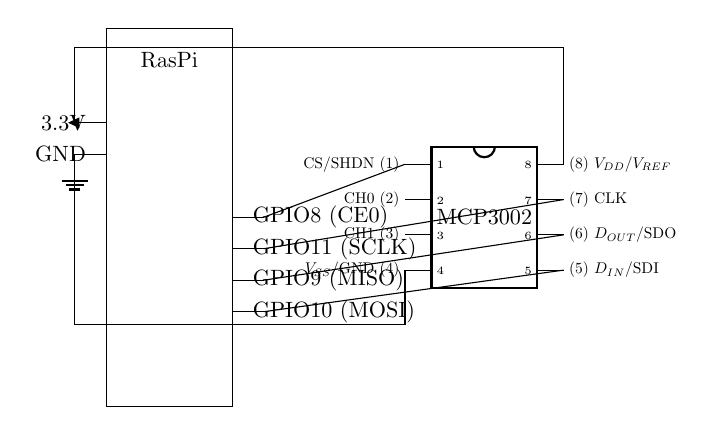
\begin{tikzpicture}[scale=0.8, transform shape]
    \ctikzset{label/align = smart}

    % Raspberry Pi (Simplified) - Same as above
    \draw (0,0) rectangle (2,6);
    \node at (1,5.5) {RasPi};

    \node[anchor=east] at (-0.2, 4.5) {3.3V}; \draw (0,4.5) -- ++(-0.5,0) node[currarrow,rotate=180]{};
    \node[anchor=east] at (-0.2, 4.0) {GND}; \draw (0,4.0) -- ++(-0.5,0) node[ground]{};

    \node[anchor=west] at (2.2, 3.0) {GPIO8 (CE0)}; \draw (2,3.0) -- ++(0.5,0);
    \node[anchor=west] at (2.2, 2.5) {GPIO11 (SCLK)}; \draw (2,2.5) -- ++(0.5,0);
    \node[anchor=west] at (2.2, 2.0) {GPIO9 (MISO)}; \draw (2,2.0) -- ++(0.5,0);
    \node[anchor=west] at (2.2, 1.5) {GPIO10 (MOSI)}; \draw (2,1.5) -- ++(0.5,0);

    % MCP3002 (DIP-8 style) - Same as above
    \node (mcp3002) [dipchip, num pins=8, external pins width=0.3] at (6,3) {MCP3002};
    \node[anchor=east, scale=0.7] at (mcp3002.pin 1) {CS/SHDN (1)};
    \node[anchor=east, scale=0.7] at (mcp3002.pin 2) {CH0 (2)};
    \node[anchor=east, scale=0.7] at (mcp3002.pin 3) {CH1 (3)};
    \node[anchor=east, scale=0.7] at (mcp3002.pin 4) {$V_{SS}$/GND (4)};
    \node[anchor=west, scale=0.7] at (mcp3002.pin 5) {(5) $D_{IN}$/SDI};
    \node[anchor=west, scale=0.7] at (mcp3002.pin 6) {(6) $D_{OUT}$/SDO};
    \node[anchor=west, scale=0.7] at (mcp3002.pin 7) {(7) CLK};
    \node[anchor=west, scale=0.7] at (mcp3002.pin 8) {(8) $V_{DD}$/$V_{REF}$};

    % Connections: Raspberry Pi to MCP3002 - Same as above
        % Route 3.3V to VDD/VREF (pin 8)
    \draw (-0.5, 4.5) -- ++(0,1.2) node[coordinate](vcc_bus_fig2){} -| (mcp3002.pin 8);
        % Route GND to VSS/GND (pin 4)
    \draw (-0.5, 4.0) -- ++(0,-2.7) node[coordinate](gnd_bus_fig2){} -| (mcp3002.pin 4);

    \draw (2.5, 3.0) -- (mcp3002.pin 1); % CE0 to CS
    \draw (2.5, 2.5) -- (mcp3002.pin 7); % SCLK to CLK
    \draw (2.5, 2.0) -- (mcp3002.pin 6); % MISO to DOUT
    \draw (2.5, 1.5) -- (mcp3002.pin 5); % MOSI to DIN

    % LM35DZ Temperature Sensor (TO-92 style representation)
    % Pinout (flat side facing, left to right): 1:Vs, 2:Vout, 3:GND
    % \node (lm35) [op amp, noinv input up, inv input down, anchor=out, scale=0.7, nofill] at (8.5, 2.5) {};
    % \node[above left=0.05cm and -0.2cm of lm35.+, scale=0.7] {$V_S$ (1)};
    % \node[above right=0.05cm and -0.2cm of lm35.-, scale=0.7] {GND (3)};
    % \node[right=0.1cm of lm35.out, scale=0.7] {$V_{OUT}$ (2)};
    % \node at (lm35.south) [below=0.1cm, scale=0.8] {LM35DZ};

    % % Connections for LM35DZ
    %     % Connect Vs (Pin 1 of LM35) to 3.3V line from RasPi
    % \draw (vcc_bus_fig2) -- ++(2.5,0) |- (lm35.+);
    %     % Connect GND (Pin 3 of LM35) to GND line from RasPi
    % \draw (gnd_bus_fig2) -- ++(2.5,0) |- (lm35.-);
    %     % Connect Vout (Pin 2 of LM35) to CH0 of MCP3002
    % \draw (lm35.out) -- ++(0.5,0) |- (mcp3002.pin 2);

    % CH1 not connected or to GND (showing not connected)
    % \draw (mcp3002.pin 3) -- ++(-0.3,0) node[xmittale, scale=0.5]{}; % NC symbol
   
    \end{tikzpicture}
    \caption{演習3 回路図 (MCP3002 と LM35DZ 温度センサ)}
    \label{fig:exercise3_updated}
\end{figure}

\subsection{プログラム}
ソースコード\ref{exam5-3}にアナログ温度センサ LM35DZ の測定を行ったプログラムを示す。
このコードでは、ADコンバータを使用して温度センサの出力電圧を測定している。
コンバータから取った値に対して入力電圧を掛けてから1023で割ることで、実際の電圧を求めている。
その後、温度センサの出力電圧を10mV/℃で割ることで、温度を求めている。

\subsection{実行結果}
以下に実行結果を示す。
\begin{table}[htbp]
    \centering
    \caption{温度センサ LM35DZ の測定結果}
    \begin{tabular}{|c|c|c|}
        \hline
        \textbf{測定日時} & \textbf{測定環境} & \textbf{測定温度 [℃]} \\
        \hline
        2025/05/22 16:00 & 温風を遠くから当てた状態 & 30.6 \\
        \hline
        2025/05/22 16:30 & 室内(エアコン使用) & 20.2 \\
        \hline
        2025/05/22 17:00 & 室内(窓開放) & 23.2 \\
        \hline
    \end{tabular}
    \label{tab:temperature_results}
\end{table}

\noindent
表\ref{tab:temperature_results}は、様々な環境での温度センサの測定結果を示している。
LM35DZセンサは、環境の変化に応じて出力電圧が変化し、それに比例して温度表示も変化することが確認できた。
特に、手で温めた場合は体温に近い値を示し、センサの応答性の高さが確認できた。

\section{演習3 - 問い}
\begin{shaded}
    \noindent
    センサ温度->センサ出力->AD変換結果->温度表示の流れを示す。
\end{shaded}

センサ温度からAD変換を経て温度表示までの流れを、以下のように示す。

\subsection*{変換プロセスの説明}
1. \textbf{環境温度 → センサ出力}:\\
   LM35DZセンサは環境温度を検知し、10mV/℃の比率で出力電圧に変換する。\\
   例:25℃の環境では、$V_{out} = 0.01 \times 25 = 0.25$ [V]となる。

2. \textbf{センサ出力 → AD変換結果}:\\
   MCP3002 ADコンバータは、入力された電圧を10ビット(0-1023)のデジタル値に変換する。\\
   変換式:$D = V_{out} \times \frac{1023}{V_{ref}}$($V_{ref}$は基準電圧で3.3V)\\
   例:0.25Vの入力では、$D = 0.25 \times \frac{1023}{3.3} \approx 77.5$となる。

3. \textbf{AD変換結果 → 温度表示}:\\
   デジタル値から再び電圧を計算し、それを温度に変換する。\\
   変換式:$T' = \frac{D \times V_{ref}}{1023} \div 0.01$\\
   例:デジタル値77.5では、$T' = \frac{77.5 \times 3.3}{1023} \div 0.01 = 25$ [℃]となる。

この変換過程により、センサが検知した環境温度が正確に表示される。

\newpage

\lstinputlisting[caption={演習2 コード}, label={exam5-2}]{c:/Program_Code/Python/BuiltIn/exam5-2.py}
\lstinputlisting[caption={演習3 コード}, label={exam5-3}]{c:/Program_Code/Python/BuiltIn/exam5-3.py}

\end{document}